
%%%%%%%%%%%%%%%%%%%%%%% file typeinst.tex %%%%%%%%%%%%%%%%%%%%%%%%%
%
% This is the LaTeX source for the instructions to authors using
% the LaTeX document class 'llncs.cls' for contributions to
% the Lecture Notes in Computer Sciences series.
% http://www.springer.com/lncs       Springer Heidelberg 2006/05/04
%
% It may be used as a template for your own input - copy it
% to a new file with a new name and use it as the basis
% for your article.
%
% NB: the document class 'llncs' has its own and detailed documentation, see
% ftp://ftp.springer.de/data/pubftp/pub/tex/latex/llncs/latex2e/llncsdoc.pdf
%
%%%%%%%%%%%%%%%%%%%%%%%%%%%%%%%%%%%%%%%%%%%%%%%%%%%%%%%%%%%%%%%%%%%


\documentclass[runningheads,a4paper]{llncs}

\usepackage{amssymb}
\setcounter{tocdepth}{3}
\usepackage{graphicx}
\graphicspath{{images/}}
\usepackage{url}
\urldef{\mailsa}\path|{chen jie}@bit.edu.cn|    
\newcommand{\keywords}[1]{\par\addvspace\baselineskip
\noindent\keywordname\enspace\ignorespaces#1}

\begin{document}

\mainmatter  % start of an individual contribution

% first the title is needed
\title{Event Timeline Summarization Using Aging Theory and Incremental Latent Semantic Analysis}

% a short form should be given in case it is too long for the running head
\titlerunning{Event Timeline Summarization Using Aging Theory and Incremental LSA}

% the name(s) of the author(s) follow(s) next
%
% NB: Chinese authors should write their first names(s) in front of
% their surnames. This ensures that the names appear correctly in
% the running heads and the author index.
%
%\author{Jie Chen \and Changmin Zhang \and Yulong Shi \and Zhendong Niu}


\authorrunning{Lecture Notes in Computer Science: Authors' Instructions}
% (feature abused for this document to repeat the title also on left hand pages)

% the affiliations are given next; don't give your e-mail address
% unless you accept that it will be published
%\institute{Springer-Verlag, Computer Science Editorial,\\
%Tiergartenstr. 17, 69121 Heidelberg, Germany\\
%\mailsa\\
%\mailsb\\
%\mailsc\\
%\url{http://www.springer.com/lncs}}

%
% NB: a more complex sample for affiliations and the mapping to the
% corresponding authors can be found in the file "llncs.dem"
% (search for the string "\mainmatter" where a contribution starts).
% "llncs.dem" accompanies the document class "llncs.cls".
%

%\toctitle{Lecture Notes in Computer Science}
%\tocauthor{Authors' Instructions}
\maketitle


\begin{abstract}
\emph{To reduce people’s time for obtaining the valuable information from amounts of web news, many summarization approaches have been researched. However, most of these approaches ignore the temporal characteristics of news reporting a same event. In this paper, we focus on summarizing the development and changes of events by taking timeline and semantic into consideration. There are three steps in our method. First, we extract hot terms from news which report the same event according to their energy during the time interval we choose (i.e. one day). Second, we use an incremental latent semantic analysis model to recognize the semantic units of news. Third, we construct a semantic text relationship map and choose sentences both important and diverse to generate timeline summaries. Experiment results show that our method can improve the timeline summarization significantly.}

\keywords{Summarization, timeline, aging theory, incremental LSA}
\end{abstract}
\section{Introduction}

Everyday thousands of news stories reporting different events are published on the Internet. These reports are disordered and people have to read most of them to know what is happening which is a time-consuming job undoubtedly. How can we get useful information about an event efficiently? Automatic summarization has been such a method solving this kind of information overloading since Luhn \cite{1958-Luhn-p159-165} proposed it in 1958. And numerous pages have been published in the field, ranging from single document to multiple documents, from extraction to abstraction, from traditional document to web document, email, blog and other types of genre. However, these research work focus on the central idea of document or document set ignoring the temporal characteristics of events. As a result, people cannot catch the changes of events over time efficiently. 

Recent years, topic detection and tracking (TDT) which detects new events from the large scale news stream and tracks them as events going on draws researchers' attention. But it did not display events properly, and people still have to read all the relevant reports to get what they want to know about the event. However, we are still enlightened by its usage of tracking which make us decide to generate a timeline summary consisting of a series of individual small summaries with sentences both important and diverse to help people understand the development of an event more quickly.

Every event goes through a life cycle of birth, growth, maturity and death, which means that special terms utilized for descripting different events experience a similar life cycle. Aging theory \cite{2003-Chen-p47-59} is a model exploited in event detection task which tracks life cycles of events using energy function. The energy of an event increases when the event becomes popular, and it diminishes with time. In our opinion, it can also be used for summarization to help us find out the daily hot terms of events. Then people can obtain what new changes happen as events going on.

The importance of sentences is decided by terms occurring at the documents in keywords-based summarization. But different authors use different words to express a same meaning and many words has several meanings. So identifying the implicit semantics of news can improve summary quality greatly. Here, we propose an incremental model based on latent semantic analysis (LSA) \cite{1990-Deerwester-p391-407} which is a robust unsupervised technique for deriving an implicit representation of text semantics based on observed co-occurrence of words to find semantic units of news.

As descripted above, in this paper, we generate news event summary by considering both temporal and semantic characteristics. We first utilize the aging theory \cite{2003-Chen-p47-59} to extract hot terms from news which reports the same event according to their energy during the time interval we choose (i.e. one day). Then we identify the semantic units of news with the incremental latent semantic analysis model. Last, we construct a semantic text relationship map, choose sentences which are both important and novel to form the summary and display them using a timeline so that people can track event trajectory easily and quickly.

The remainder of this paper is organized as follows: Section 2 reviews some related works on summarization. We discuss our approach of event timeline summarization using aging theory and incremental latent semantic analysis model in section 3. Our experiments and some discusses are described in section 4. Section 5 presents our conclusions and some future plans.

\section{Related Work}

It has been more than 50 years since Luhn \cite{1958-Luhn-p159-165} proposed automatic summarization. During these years numerous papers have been published on this topic and it has been adopted in many fields. In the beginning, researchers focus on single document summarization. With the rapid development of Internet, the amount of information is increasing in an exponential manner and people easily get lost when faced with such overwhelming information. In order to resolve this kind of information overload, multi-document summarization has attracted researchers' eyes. Centroid-based method is one of the most popular multi-document summarization methods generating summaries using centroids, position and first-sentence overlapping \cite{2004-Radev-p919-938}. While in clustering approaches researchers cluster similar sentences together and select one representative sentence from each main cluster \cite{1997-Salton-p193-207,2005-Harabagiu-p202-209}. Later, machine learning \cite{2008-Wong-p985-992} and graph-based method \cite{2004-Erkan-p365-371,2005-Mihalcea-p-} are exploited to multi-document summarization. But they all did not consider temporal characteristic.
Swan et al. \cite{2000-Swan-p49-56} presented temporal characteristics while displaying events under the task of Topic Detection and Tracking. Allan et al. \cite{2001-Allan-p10-18} built a temporal summary of news stories to help people monitor changes in news coverage over time. Chieu et al. \cite{2004-Chieu-p425-432} generated a timeline summary combing a series of events related to an entity with interest and burstiness. Yan et al.\cite{2011-Yan-p745-754} built a query-based evolutionary timeline summarization via a balanced optimization framework considering four attributes. However, they all missed the daily hot points of events. Aging theory was put forward by Chen et al. \cite{1990-Deerwester-p391-407} in the task of hot topic detecting, and now we transfer it to our timeline summarization to solve this problem.

In order to improve the qualities of summaries, Brunn et al. \cite{2001-Brunn-p-} proposed to utilize lexical chain to identify the semantic units. Concepts were also exploited to summarization task by \cite{2007-Ye-p1643-1662}. But they all had a heavy reliance on WordNet \cite{1990-Miller-p235-244}. Yeh et al. \cite{2001-Gong-p19-25} use latent semantic analysis to document summarization without the dependency on lexical resources. Inspired by Yeh, we propose an incremental LSA model for our timeline summarization. 


\section{Our Approach}

\subsection{Hot terms identification using Aging Theory}

Aging theory is a technique used for tracking life cycles of events, for it consider that every event has a life form with stages of birth, growth, decay and death \cite{2003-Chen-p47-59}. Since terms or words are the basic elements of any news report, changes in the content of reports will be reflected by variations in the usage of terms \cite{2007-Chen-p1016-1025}. When a new change of an event occurred, several pieces of news will report it using some special words that can reflect the new change, so frequencies of these words will increase greatly, and with the change’s popularity wanes, the frequencies will decrease accordingly. So terms have a similar life span to events, and we can use aging theory to track terms to determine what life stage they are in. Further, we can find out the daily hot spots to improve our summarization.

As aging theory using the concept of energy to indicate the liveliness of an event in its life span, our first step is to calculate the energy of terms. The frequency of a word will change as event going on, so we use the association between word  and time interval  to indicate its energy which is defined as follows:
\begin{equation}
  E_{w,t} =F(F^{-1}E_{w,t-1}+\alpha\cdot\chi^2_{w,t})
\end{equation}
where $E_{w,t}$ is the energy of word $w$  in time interval $t$ , and $E_{w,t-1}$  is the energy of word $w$ in time interval $t-1$ , $\alpha$ is the transfer factor, and $\chi^2_{w,t}$  is the contribution degree of word  at the time interval $t$, which can be computed as presented in \cite{2000-Swan-p49-56}. 

However, no words descripting a special event point will retain popular forever, they will decay over time. In order to represent the word's life span realistically, we cut down the energy of word by a decay factor β at the end of every time interval. And if the decayed energy value became negative, we change it to 0.

According to the description above, if the energies of some words increase greatly, we can draw a conclusion that there is a hot event spot. So we need to calculate the variance of word energy next. Here we use standard deviation:
\begin{equation}
Var_{w,t} = \sqrt{ \frac{1}{N} \sum_{t \in period}(E_{w,t}- \overline{E_{w}})^2}
\end{equation}
where $N$ is the number of time intervals during the given period, $E_{w,t}$  is the energy of word $w$  in time interval $t$ , $\overline{E_{w}}$  is the average energy during the period, and $Var_{w,t}$  is the variance of $w$ .
Then each word will be assigned a new weight besides the traditional TFIDF which can be defined as:
 \begin{equation}
NewWeight(w)=TF*IDF_{w} + \mu \cdot Var_{w}
\end{equation}
This kind of new weight can help us identify both central and hot information, so people can capture the main line and new changes of events simultaneously.

\subsection{An incremental LSA Model}
\label{lsasection}
Here we use a variant of latent semantic analysis (LSA), a mathematical technique, to derive implicit semantics from news. The process starts with the construction of a word-by-sentence matrix A, where each row indicates a word, each column indicates a sentence, and   indicates the weight of word   in sentence , which is defined as below. Since every word does not normally appear in each sentence, the matrix A is usually sparse.

\begin{displaymath}
A = 
\left( \begin{array}{cccc}
a_{11} & a_{12} & \ldots & a_{1n} \\
a_{21} & a_{22} & \ldots & a_{2n} \\
\vdots & \vdots & \ddots & \vdots \\
a_{m1} & a_{m2} & \ldots & a_{mn}
\end{array} \right)
\end{displaymath}

We then apply the singular value decomposition (SVD) to the matrix A, which is defined as:
\begin{equation}
A = U \Sigma V^T
\end{equation}
where U is an $m×n$ matrix whose columns are called left singular vectors, $\Sigma$ is an $n×n$ diagonal matrix whose diagonal elements are non-negative singular values sorted in descending order, and V is an $n×n$ matrix whose columns are called right singular vectors.
Next, we perform a dimension reduction to the diagonal matrix $\Sigma$ by cutting down some elements in it and we get matrix $\Sigma '$. Then a new matrix $A'$ is reconstructed by multiplying three matrices as:
\begin{equation}
A' = U' \Sigma V'^T \approx A
\end{equation}
 where $\Sigma'$ represents the semantic space that can derive latent semantic structures from A, U' and V' is the dimension reduced matrices correspond to U and V respectively. Each column of A' denotes the semantic sentence representation, and each row denotes the semantic word representation.

Since we generate a small summary every day during the life cycle of event, we should know information not only on that day but also on its previous neighbors for we do not know what will happen in the future. So if a new news set come, we need to combine them with the previous obtained semantic space so as to acquire more precise data. Firstly, we find out new words compared to previous neighbors and append them to the word-by-sentence matrix as well as new sentences. And the   for the new comers is the term weight on that day as blow: 
\begin{displaymath}
A =  \left( \begin{array}{cccc}
				&	a_{1n_1}	 &	 \ldots 	& a_{1n_N} 	\\
A'				& 	\vdots 	&	\ddots 	& \vdots 		\\
				& 	a_{mn_1} & 	\ldots 	& a_{mn_N}	\\

				& a_{m_1n_1} & 	\ldots 	& a_{m_1n_N} \\
0				& 	\vdots 	& 	\ddots 	& \vdots 		\\
				& a_{m_Mn_1} &   \ldots 	&a_{m_Mn_N}
\end{array}\right)
\end{displaymath}
where $A'$ is the semantic space obtained before that date, $0$ indicates the weight of new words in old sentences since they did not occur , while others are the weight of words in the new sentences.  
Then we can perform the same latent semantic analysis process to the incremental matrix with the description above and get a new semantic space at a wider range.

\subsection{Summary generation}
We generate our timeline summary with two metrics: importance and diversity. Importance means summary sentences must represent the main information about the event. Diversity means we need select sentences novel enough compared to sentences both on that day and on other days.

\subsubsection{Importance metric}
We use a graph-based method to determine sentence importance score. Each node in the graph stands for a semantic sentence and is represented by a vector of semantic words obtained in section ~\ref{lsasection}. The edge between two nodes is weighted by the similarity value between two sentences which is calculated by cosine similarity:
\begin{equation}
sim(\overrightarrow{s_i}, \overrightarrow{s_j}) = \frac{\overrightarrow{s_i} \cdot \overrightarrow{s_j} } {| \overrightarrow{s_i} || \overrightarrow{s_j} |}
\end{equation}

And then, the importance of sentence $s$ is measured by the average similarities between $s$ and all the other sentences in the news set:
\begin{equation}
importance(s_i) = \frac{1}{n-1} \sum_{j=0, j \neq i}^n sim(\overrightarrow{s_i}, \overrightarrow{s_j})
\end{equation}
where $n$ is the number of sentences.

\subsubsection{Diversity metric}
Since our purpose is to generate a timeline summary consisting of an individual small summary per day, we should also consider diversity of sentences to minimize the redundancy between sentences today and the produced small summaries on previous days, which is called cross-date diversity. Here we also use cosine similarity to measure the diversity but unlike the usual idea of similarity, diversity means the distance between s and the previous summary, so smaller similarity value is expected:
\begin{equation}
diversity(s) = sim(s, sum)
\end{equation}
where   $sum$ is the small summary produced before the date sentence $s$ belonging to for if we use all the existing summaries, there may be a topic excursion and some new changes related to prior information may be filtered out. Here sentence s and summary is also represented by the vector of the semantic words obtained in section ~\ref{lsasection}.

\subsubsection{Sentence selection}

For importance bigger similarity value is desired while for diversity we need smaller similarity value. Here we introduce two decreasing/increasing logistic functions,  $L_1(x) = 1/(1+e^x)$  and $L_2(x) = e^x / (1+e^x)$ , like \cite{2011-Yan-p745-754} to balance importance and diversity. And finally we can combine the two measure metrics together to determine sentence weight:
\begin{equation}
weight(s) = \lambda \cdot L_2 \cdot importance(s) + (1- \lambda ) \cdot L_1 \cdot  diversity(s)
\end{equation}

However, simply ranking sentences based on the weighted score above may result in similar sentences at the top of list, so we still utilize MMR \cite{1998-Carbonell-p335-336} to avoid sentences having similar meanings on the same day both presenting.

\section{Experiments and dicussions}
\subsection{Dataset}
Here we use dataset from TAC2010 which contains 46 events taken from the New York Times, the Associated Press, the Xinhua News Agency newswires, and the Washington Post News Service. Since our experiment is based on the timeline which can track the development of events and there are no standard summaries for timeline summarization evaluation, we generate a timeline summary for each event manually and save it as the standard. Here we take 5 events as examples.
\subsection{Experiment}
\label{methodsection}

We start our experiment with some preprocessing like indexing, filtering out the stop words and segmenting news documents into sentences. Then we perform our method to the data set and generate a timeline for each event we choosing. We also implement some widely used multi-document summarization methods as the baselines.

$Centroid$ extracts sentences based on centroid value, positional value and first-sentence overlap.

$Cluster$ considers that there are different themes in an event, so it first clusters similar sentences together into different clusters and then selects one representative sentence from each main cluster.

$Allan$ is a similar timeline system from different aspect proposed by Allan et al., dividing sentences into on-event and off-event while ranking them with useful and novelty.

We also compared our method with itself in the aspect of considering aging theory and the incremental latent semantic analysis or not to enhance our thesis.

\subsection{Evaluation Metrics}
Here we use ROUGE toolkit \cite{2004-Lin-p74-81} , which is officially applied by Document Understanding Conference (DUC) for document summarization performance evaluation, to evaluate the experimental results and compare these algorithms with each other. The summarization quality is measured by counting the number of overlapping units, such as N-gram, word sequences, and word pairs between the auto-generated summary and the manual summary. Several automatic evaluation methods are implemented in ROUGE, such as ROUGE-N, ROUGE-L and ROUGE-W, each of which can generate three scores (recall (R), precision (P) and F-measure). Take ROUGE-N as an example:

\begin{equation}
R=\frac{\sum_{s \in manual } \sum_{N-gram \in s} Count_{match}(N-gram) } { \sum_{s \in manual} \sum_{N-gram \in s} Count(N-gram)  } \end{equation}
\begin{equation}
P=\frac{\sum_{s \in auto } \sum_{N-gram \in s} Count_{match}(N-gram) } { \sum_{s \in auto} \sum_{N-gram \in s} Count(N-gram)  }
\end{equation}
\begin{equation}
F-measure = \frac{2PR}{P+R}
\end{equation}

Where $N$ stands for the length of the $N-gram$, $Countmatch(N-gram)$ is the maximum number of N-grams co-occurring in the auto-generated summary and the manual summary. Here we execute our evaluation in terms of ROUGE-1. And since our summary consists of a series of individual small summaries, we use the average ROUGE score as the final score.

\subsection{Results and discussions}
We compared our proposed method AIL and some other widely used approaches descripted in section~\ref{methodsection} as well as the methods without aging theory (AIL1) or incremental LSA (AIL2) to the events and the overall results are shown in Fig ~\ref{fig:zhuzhuangtu}. Table ~\ref{evalutions} describes some details about the results of the 5 example events.
\begin{figure}
\centering
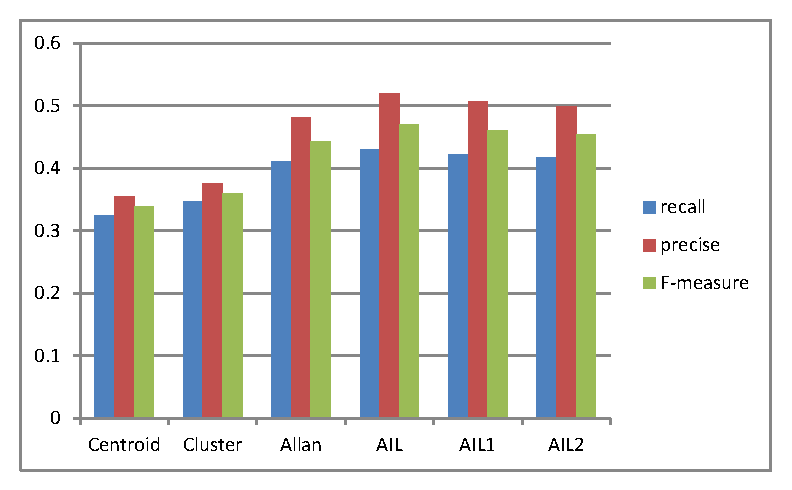
\includegraphics[height=6.2cm]{zhuzhuangtu}
\caption{Overall performance of these approaches}
\label{fig:zhuzhuangtu}
\end{figure}

\begin{table*}
\centering
\caption{Evalution results of the five events }
\begin{tabular}{c|c c c c c c c}
\hline
                  &             		& $Centroid$ & $Cluster$ & $Allan$    & $AIL$       & $AIL_1$    & $AIL_2$ \\
\hline
                 &  recall		& 0.3641     & 0.3639 & 0.3967 & 0.4258 & 0.4186 & 0.4098 \\
Event1   &  precision	& 0.3789     & 0.3867 & 4939    & 0.5190 & 0.5046 & 0.4962 \\
	       &  F-measure	& 0.3713     & 0.3749 & 0.4399 & 0.4678 & 0.4575 & 0.4488 \\
\hline
                 &  recall 		& 0.3201     & 0.3540 & 0.4029 & 0.4230 & 0.4146 & 0.4115 \\
Event2   &  precision	& 0.3538     & 0.3730 & 0.4940 & 0.5238 & 0.5068 & 0.5032 \\
	       &  F-measure 	& 0.3361     & 0.3632 & 0.4438 & 0.4680 & 0.4560 & 0.4527 \\
\hline
                 &  recall 		& 0.3273     & 0.3736 & 0.4136 & 0.4330 & 0.4238 & 0.4189 \\
Event3   &  precision	& 0.3523     & 0.3846 & 0.4846 & 0.5297 & 0.5153 & 0.4911 \\
	       &  F-measure 	& 0.3393     & 0.3790 & 0.4462 & 0.4764 & 0.4651 & 0.4521 \\
\hline
                 &  recall 		& 0.3112     & 0.3264 & 0.4292 & 0.4492 & 0.4380 & 0.4338 \\
Event4   &  precision	& 0.3384     & 0.3692 & 0.4664 & 0.5130 & 0.5068 & 0.5029 \\
	       &  F-measure 	& 0.3242     & 0.3465 & 0.4470 & 0.4789 & 0.4698 & 0.4658 \\
\hline
                 &  recall 		& 0.3001     & 0.3153 & 0.4153 & 0.4201 & 0.4183 & 0.4168 \\
Event5   &  precision	& 0.3540     & 0.3679 & 0.4679 & 0.5162 & 0.5048 & 0.5006 \\
	       &  F-measure 	& 0.3248     & 0.3395 & 0.4401 & 0.4632 & 0.4574 & 0.4548 \\
\hline
\end{tabular}
\label{evalutions}
\end{table*}

From the results, we can see that: $Centroid$ has the worst performance mainly because it selects sentences according to the centroids of document set which makes it capture the main points of events but loses the coverage of other points. $Cluster$ divides sentences with different meanings into different clusters and selects one representative sentence from each cluster which improves its overall performance but still works worse than $Allan$ and our methods due to neglecting the temporal characteristics. For $Allan$, it ranks sentences with useful and novelty and take into account timeline so it outperforms $Centroid$ and $Cluster$. And unsurprisingly, our proposed method outperforms all these baselines, indicating that aging theory and incremental $LSA$ is applicable to timeline summarization. Comparison within our approach enhances our proposition further for without either aging theory or incremental $LSA$ the performance will drop obviously.
In order to balance importance and diversity metrics when combine them together in Eq.9, we change the parameter λ from 0.1 to 0.9. And its effect on the results is shown in Fig \ref{fig:lambda}.

\begin{figure}
\centering
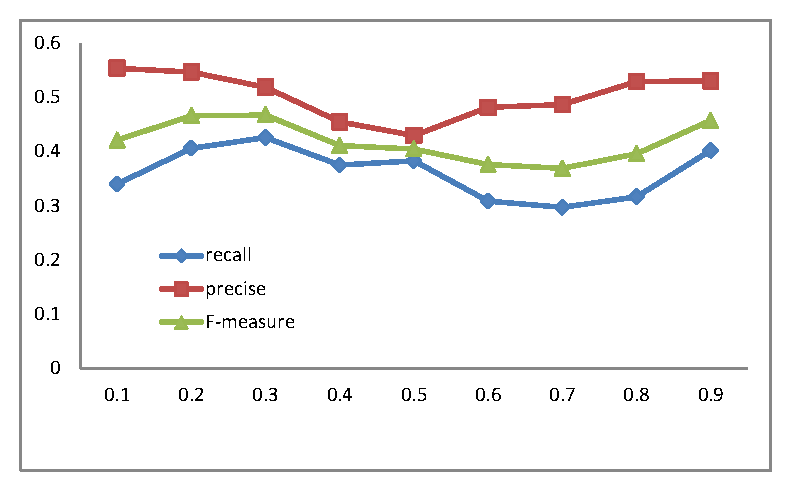
\includegraphics[height=6.2cm]{lambda}
\caption{The effect of $\lambda$ on the results when ranging from 0.1 to 0.9}
\label{fig:lambda}
\end{figure}

From Figure 2 we can see that when $\lambda$=0.3 our approach receive the best performance, indicating that in timeline summarization which emphasizes new changes as the event going on we should bias to diversity slightly.

\section{Conclusion}
In this paper, we present a novel approach for event timeline summarization. In our approach, we firstly identify hot terms on every day during the life cycle of the event using aging theory. Then we recognize the implicit semantics from news set with incremental $LSA$. At last sentences both important and diverse are selected with a graph-based method and a timeline consisting of a series of individual small summaries which can represent the development trajectory of event is constructed. Experiment results show that our approach performs better compared with other widely used methods.

In the future, we will identify semantic units using other methods for $LSA$ can process synonym but is unable to handle polysemy. And we will also extend our approach to short text such as microblogs and comments.

\bibliographystyle{ieeetr}
\bibliography{../../bib/text_summary}

\end{document}
